\documentclass[12pt,a4paper]{report}

\usepackage{enumitem} % control over list


%=======================================================%
%   Compact Table of Contents, Figures, and Tables
%=======================================================%

\usepackage{tocloft} 
% TOC spacing
\setlength{\cftbeforetoctitleskip}{0pt}
\setlength{\cftaftertoctitleskip}{15pt}

% List of Figures spacing
\setlength{\cftbeforeloftitleskip}{0pt}
\setlength{\cftafterloftitleskip}{15pt}

% List of Tables spacing
\setlength{\cftbeforelottitleskip}{0pt}
\setlength{\cftafterlottitleskip}{15pt}  


%=======================================================%
%           General Formatting
%=======================================================%
\setlength{\parindent}{0pt}  
\setlength{\parskip}{6pt} 
% \pagenumbering{arabic}% Page Number

\begin{document}

%=======================================================%
%       Cover Page
%=======================================================%
\begin{center}

\vspace{1cm}

{\LARGE \textbf{Enhanced Urban Mobility through Deep Learning Based Real-Time Passenger Head Counting and Occupancy Estimation }}

\vspace{1.5cm}

{\large \textbf{Project Type:} Research Based Project}

\vspace{2.5cm}

\textbf{Submitted By}

\vspace{1cm}

{\large \textit{Name: Md Masum Billah}}

\vspace{0.3cm}

Student ID: ASH2125033M

\vspace{0.3cm}

Session: 2020-2021

\vspace{2.5cm}

\textbf{Supervisor }

\vspace{0.5cm}

{\large \textit{Name: 
Nazmun Nahar}}

\vspace{0.3cm}

Designation: Assistant Professor

\vspace{3cm}

\textbf{Software Engineering Program (BSc. Hons.)}\\
Institute of Information Technology (IIT)\\
Noakhali Science and Technology University

\vspace{2.5cm}

\textbf{Submission Date:} 13/08/2026

\end{center}


% ============================================================
% SIGNATURE PAGE (Student and Supervisor)
% ============================================================
\newpage
\phantomsection
\addcontentsline{toc}{chapter}{Declaration}
\thispagestyle{empty}
\begin{center}
    \Large\textbf{Declaration}
\end{center}
\vspace{1cm}

\noindent This is to certify that the thesis titled \textbf{``Enhanced Urban Mobility through Deep Learning Based Real-Time Passenger Head Counting and Occupancy Estimation''}
submitted by \textbf{Md Masum Billah} (ID: ASH2125033M) has been carried out under my
supervision and is approved for submission.

\vspace{3cm}

\noindent
\begin{minipage}[t]{0.45\textwidth}
    \rule{6cm}{0.4pt}\\
    \textbf{Md Masum Billah}\\
    ASH2125033M\\
    Institute of Information Technology (IIT)
\end{minipage}
\hfill
\begin{minipage}[t]{0.45\textwidth}
    \rule{6cm}{0.4pt}\\
    \textbf{Nazmun Nahar}\\
    Supervisor, Assistant Professor\\
    Institute of Information Technology (IIT)
\end{minipage}


% ============================================================
% DEDICATION
% ============================================================
\newpage
\phantomsection
\addcontentsline{toc}{chapter}{Dedication}
\thispagestyle{empty}
\vspace*{5cm}
\begin{center}
    \textit{Dedicated to my beloved parents}
\end{center}


% ============================================================
% APPROVAL (Exam Committee)
% ============================================================
\newpage
\phantomsection
\addcontentsline{toc}{chapter}{Approval}
\thispagestyle{empty}
\begin{center}
    \Large\textbf{Approval}
\end{center}
\vspace{1cm}

\noindent The thesis titled \textbf{``Enhanced Urban Mobility through Deep Learning Based Real-Time Passenger Head Counting and Occupancy Estimation''} submitted by
\textbf{Md Masum Billah} (ID: ASH2125033M) has been accepted as satisfactory in partial
fulfillment of the requirements for the degree of \textbf{BSc. (Hons.) in Software Engineering} on
[Date of Defense].

\vspace{1cm}
\noindent\textbf{Board of Examiners}

\vspace{2cm}
\noindent
\rule{6cm}{0.4pt}\\
\textbf{[Name]}\\
Chairman\\
[Designation, Department]

\vspace{2cm}
\noindent
\rule{6cm}{0.4pt}\\
\textbf{[Name]}\\
Member (Internal)\\
[Designation, Department]

\vspace{2cm}
\noindent
\rule{6cm}{0.4pt}\\
\textbf{[Name]}\\
Member (External)\\
[Designation, Department]

% ============================================================
% ACKNOWLEDGEMENT
% ============================================================
\newpage
\phantomsection
\addcontentsline{toc}{chapter}{Acknowledgement}
\thispagestyle{empty}
\begin{center}
    \Large\textbf{Acknowledgement}
\end{center}
\vspace{1cm}

\noindent I would like to express my sincere gratitude to my supervisor,
\textbf{Nazmun Nahar}, for her invaluable guidance, patience, and support
throughout this research. I am also thankful to the faculty members of the
Institute of Information Technology (IIT) for their encouragement.

I extend my heartfelt thanks to my family and friends for their unwavering support
and motivation during this journey.

% ============================================================
% ABSTRACT (150-250 words)
% ============================================================
\newpage
\phantomsection
\addcontentsline{toc}{chapter}{Abstract}
\thispagestyle{empty}
\begin{center}
    \Large\textbf{Abstract}
\end{center}

\noindent
Write your abstract here. It should briefly cover the background/motivation of the
study, the problem statement, the methodology used, key findings, and the
significance/contribution of the work. Keep the total length between 150 and 250
words, written as a single, self-contained paragraph without citations.

\clearpage

% --------------------------------------------------
% Table of Contents
% --------------------------------------------------
\renewcommand{\contentsname}{Table of Contents}
\tableofcontents
\clearpage

% --------------------------------------------------
% List of Figures
% --------------------------------------------------
\listoffigures
\addcontentsline{toc}{chapter}{List of Figures}
\clearpage

% --------------------------------------------------
% List of Tables
% --------------------------------------------------
\listoftables
\addcontentsline{toc}{chapter}{List of Tables}
\clearpage

% ============================================================
% LIST OF ABBREVIATIONS
% ============================================================
\newpage
\phantomsection
\addcontentsline{toc}{chapter}{List of Abbreviations}
\begin{center}
    \Large\textbf{List of Abbreviations}
\end{center}
\vspace{1cm}

\noindent
\begin{tabular}{ll}
    \textbf{Abbreviation} & \textbf{Full Form} \\[0.3cm]
    AI   & Artificial Intelligence \\
    ML   & Machine Learning \\
    CNN  & Convolutional Neural Network \\
    YOLO & You Only Look Once \\
    IoU  & Intersection over Union \\
    mAP  & Mean Average Precision \\
    FPS  & Frames Per Second \\
    % Add more rows as needed
\end{tabular}

\clearpage

% ==================================================
% CHAPTER 1
% ==================================================
\refstepcounter{chapter}
\chapterpage{Introduction}
\mychapter{Introduction}
\section{Background and Motivation}

Public transportation systems constitute a critical pillar of modern urban infrastructure. Among all transit modes, buses serve the largest share of daily commuters worldwide, particularly in rapidly urbanising developing nations \cite{itf_outlook_2023}. Accurate information regarding passenger occupancy is important for improving route planning, optimizing fleet management, monitoring overcrowding, and enhancing passenger safety.

Traditional APC systems commonly employ hardware based sensors such as infrared beams, pressure mats, or ticketing systems. Although these approaches are widely used, they often suffer from several limitations, including high installation and maintenance costs, sensitivity to environmental conditions, and reduced accuracy when multiple passengers enter or exit simultaneously \cite{mccarthy2025video}.

Recent advancements in computer vision and deep learning have enabled the development of camera based passenger counting systems. Since many buses are already equipped with surveillance cameras for security purposes, vision based methods offer a cost effective and scalable solution \cite{McCarthy2023DeepLearning}. Deep learning models encompassing both object detection and density estimation approaches have achieved state of the art performance on crowd counting benchmarks, demonstrating that neural networks can reliably estimate occupancy in complex visual scenes.

However, bus interiors present unique challenges that distinguish them from general crowd scenes. Passengers frequently occlude each other, surveillance cameras are typically mounted on the ceiling causing perspective distortion, and passenger heads often appear as small objects in the captured images.

\section{Problem Statement}

Accurate passenger counting is a fundamental requirement for intelligent public transportation systems. Reliable passenger statistics enable transport authorities and bus operators to optimize routes, monitor occupancy levels, improve passenger safety, and make data-driven operational decisions. Conventional passenger counting systems, such as infrared sensors, pressure sensors, and ticketing-based methods, often suffer from inaccuracies due to sensor malfunction, passenger overlap, and simultaneous boarding or alighting events.

Recent advances in computer vision and deep learning have demonstrated promising results for crowd counting and object detection in surveillance applications. However, applying these methods to bus passenger counting remains challenging because of the unique characteristics of bus interiors. Passengers are often densely packed, causing severe occlusion where individuals partially or completely block one another. In addition, surveillance cameras are usually installed on the ceiling, resulting in perspective distortion and making passenger heads appear small, especially in the rear sections of the bus. Variations in illumination, motion blur caused by vehicle movement, and frequent passenger movement further complicate accurate counting.

Most existing crowd counting methods have been developed and evaluated on public datasets such as ShanghaiTech\cite{Zhu2020}, UCF-QNRF\cite{ucf_qnrf_dataset}, and NWPU-Crowd\cite{wang2020nwpu}, which mainly consist of outdoor scenes or general crowd environments. These datasets do not adequately represent the visual characteristics and challenges of bus interiors. Furthermore, many studies focus on estimating crowd density rather than identifying individual passengers across video frames, which may lead to unstable counts and double-counting problems in video-based applications.

Therefore, there is a need to investigate whether head detection can provide accurate passenger counts in bus environments, determine which detection models are most effective for detecting small passenger heads, and examine whether integrating object tracking can improve counting stability and reduce duplicate counts across frames.

\section{Research Objectives}

\subsection{General Objective}

The main objective of this study is to develop and evaluate a vision based passenger counting system for bus interiors using head detection and object tracking.

\subsection{Specific Objectives}

The specific objectives are as follows:

\begin{itemize}[itemsep=0pt]
    \item To investigate whether head detection can be used to count passengers accurately in bus interiors.
    
    \item To compare different object detection models and determine which model performs best for detecting small passenger heads in real bus scenes.
    
    \item To evaluate the effectiveness of object tracking techniques in improving counting stability and reducing double counting across video frames.
    
\end{itemize}

\section{Scope and Limitations}
\subsection{Scope}
This study focuses on the development and evaluation of a vision based passenger counting system for bus interiors using deep learning based head detection and object tracking techniques. The proposed system utilizes surveillance video captured from cameras installed inside buses to estimate the number of passengers in real time.

The scope of this study includes:

\begin{itemize}[itemsep=0pt]

\item Developing a passenger counting framework based on head detection rather than full body detection to better handle crowded bus environments and severe occlusion.

\item Evaluating and comparing multiple object detection models for detecting small passenger heads in bus surveillance videos.

\item Investigating the effectiveness of multi object tracking algorithms in maintaining passenger identities across consecutive video frames and reducing double counting errors.

% \item Assessing the performance of the proposed system using standard evaluation metrics such as Precision, Recall, mAP, MOTA, MAE, and counting accuracy.

% \item Conducting experiments on bus interior videos captured from ceiling mounted surveillance cameras under different occupancy levels and lighting conditions.

\end{itemize}

This study is limited to passenger counting inside buses and does not consider other public transportation systems such as trains, subways, or airports.

\subsection{Limitations}


Although the proposed approach aims to provide an accurate and robust passenger counting system, several limitations exist.

\begin{itemize}[itemsep=0pt]

\item The system relies on video captured from ceiling mounted surveillance cameras. Different camera positions or viewpoints may affect detection and tracking performance.

\item Severe occlusion remains a challenging problem. When passengers are completely hidden behind others, head detection may fail, leading to undercounting.

\item The performance of the tracking algorithm depends heavily on the quality of the object detector. Missed detections or false detections may cause identity switches or fragmented trajectories.

\item Variations in lighting conditions, shadows, motion blur caused by bus movement, and image quality may negatively affect the detection accuracy.

\item The proposed system assumes that the surveillance camera remains fixed. Camera movement or vibration beyond normal bus operation is not considered in this study.

\item The study focuses on passenger counting only and does not address related tasks such as passenger identification, behavior analysis, age estimation, or demographic analysis.

\end{itemize}

Despite these limitations, the study is expected to provide valuable insights into the feasibility of using head detection and object tracking for accurate passenger counting in bus environments and serve as a foundation for future research in intelligent transportation systems.


\section{Significance of the Study}


This study is significant for both academic research and practical applications. From an academic perspective, the research contributes to the growing field of vision based passenger counting by investigating the integration of head detection and object tracking in bus environments. Unlike conventional crowd counting methods that rely on density estimation, this study focuses on detecting and tracking individual passengers, thereby addressing issues such as occlusion, small object detection, and counting stability.

From a practical perspective, an accurate passenger counting system can provide valuable information for intelligent transportation systems. Real time passenger occupancy data can assist transport authorities in optimizing bus schedules, reducing overcrowding, improving service quality, and enhancing passenger safety. Furthermore, because many buses are already equipped with surveillance cameras, the proposed approach can potentially be deployed without requiring additional hardware, making it a cost effective solution for public transportation systems.

The findings of this study may also contribute to the development of smart city applications where real-time monitoring and data-driven decision-making are essential.


% ==================================================
% CHAPTER 2
% ==================================================
\refstepcounter{chapter}
\chapterpage{Literature Review}
\mychapter{Literature Review}
\section{Preliminaries}

Automatic Passenger Counting (APC) refers to the family of technologies and algorithms used to determine, in real time or near-real time, how many people board, alight, or occupy a vehicle or a defined space within a transport system. APC is a specific instance of the broader ``people counting'' or ``crowd counting'' problem, but it carries constraints that are peculiar to the transport domain: passengers move through confined doorways, they occlude one another, lighting and vibration vary with the operating environment, and any solution must eventually be installed, calibrated, and maintained on a fleet of vehicles rather than a single fixed camera.

Two broad design choices recur throughout the literature and are useful to define before reviewing individual studies.

\textbf{Invasive versus noninvasive sensing.} Invasive methods place a dedicated sensor at the point of passenger transfer---infrared beam breakers, pressure-sensitive treadles, capacitive plates, radar, or door-mounted cameras---and are generally associated with high accuracy but higher installation and maintenance cost, and in the case of cameras, closer proximity to individual passengers. Noninvasive methods instead exploit sensing infrastructure that already exists or that observes passengers indirectly (e.g., Wi-Fi probe requests, general surveillance cameras, or low-resolution depth sensors), trading some accuracy for lower cost, easier retrofit, and, in some configurations, improved privacy.

\textbf{Detection/tracking-based counting versus density-based (region-of-interest) counting.} Detection-based, or ``line-of-interest,'' methods identify individual people (or their heads) in each video frame, track them across frames, and increment a count whenever a tracked identity crosses a calibrated virtual line, typically positioned at a doorway. Density-based, or ``region-of-interest,'' methods instead regress a density or occupancy value directly from the appearance of a crowded scene without explicitly detecting or tracking every individual, and are more robust to severe occlusion at the cost of losing per-individual identity and temporal continuity. Bus-interior passenger counting research increasingly combines both paradigms, using detection for less-crowded regions and density estimation for the most congested areas of the vehicle.

These two distinctions frame nearly every design decision described in the remainder of this chapter, from camera placement and sensor modality to the choice between YOLO-style detectors, multi-object trackers, and convolutional density regressors.

\section{Relevant Theories and Concepts}

\textbf{Convolutional object detectors.} Modern vision-based APC systems are built on convolutional neural network (CNN) object detectors. The ``You Only Look Once'' (YOLO) family reframes detection as a single regression problem: an input image is divided into a grid, and each grid cell predicts a fixed number of bounding boxes together with an objectness score and class confidence, allowing bounding-box coordinates and class probabilities to be produced in a single forward pass. This end-to-end formulation, together with successors such as YOLOv3, makes the architecture attractive for real-time, edge-deployed passenger counting, since accuracy and inference speed can be traded off through model depth and input resolution. Lightweight variants such as MobileNet Single Shot Detector (SSD) pursue the same detection philosophy with a reduced parameter count, making them more suitable for low-power single-board computers of the kind typically installed on buses. A complementary line of classical detectors---Haar-cascade classifiers built from simple rectangular features and boosted with AdaBoost---remains relevant as a lightweight baseline, particularly for face and frontal head detection, although these detectors degrade quickly under partial occlusion and off-axis viewing angles.

\textbf{Crowd density estimation.} Where individual detection becomes unreliable under dense occlusion, density-map regression offers an alternative. A crowd image is labelled by placing a point (or head-position) annotation on every individual, which is converted into a continuous density map by convolving with a Gaussian kernel whose bandwidth is often scaled according to the $k$-nearest-neighbour distance between annotated points; the total count is then obtained by integrating the density map. Multi-Column CNN (MCNN) architectures address the resulting variation in apparent head size (due to camera perspective) by processing the image through parallel convolutional columns with different receptive-field sizes and fusing their outputs, while CSRNet instead achieves a large receptive field within a single column through dilated convolutions, preserving spatial resolution that multi-column architectures tend to lose through repeated pooling. Convolutional autoencoders (CAEs) have also been applied to density-based counting: an encoder--decoder network is trained to reconstruct a passenger-density representation (e.g., an inverse $k$-nearest-neighbour map) from a raw crowd image, after which the output is numerically integrated to obtain a count for a defined region.

\textbf{Multi-object tracking and re-identification.} Detection alone is insufficient for line-of-interest counting because a single passenger typically appears in many consecutive frames; tracking is required to assign a consistent identity over time and to prevent the same individual from being counted more than once. DeepSORT extends the classical SORT tracker by combining a Kalman-filter-based motion model with an appearance descriptor obtained from a re-identification network, improving robustness to short occlusions. ByteTrack instead improves association by retaining and matching low-confidence detections rather than discarding them outright, which is beneficial when passengers are partially occluded and therefore detected with lower confidence. Track--detection affinity is commonly computed from a combination of spatial overlap (Intersection-over-Union) and appearance similarity (e.g., cosine distance between re-identification feature vectors), and counting is finalised only once a tracked identity has fully traversed a calibrated region or line of interest, which helps to suppress hysteresis and false positive counts caused by people who enter and then retreat from the counting zone.

\textbf{Recurrent and sequence models for counting.} Because a passenger-counting event unfolds over a variable-length sequence of frames (the duration of a door-opening phase), recurrent architectures---particularly Long Short-Term Memory (LSTM) networks---have been proposed as an alternative to the detect-then-track pipeline. An LSTM-based counter can, in principle, learn to accumulate evidence of boarding and alighting events across an entire sequence and output a final count without any explicit detection, tracking, or background-subtraction stage, which simplifies the processing pipeline and can support very low-resolution, privacy-preserving sensor inputs.

\textbf{Evaluation metrics.} Across the reviewed literature, counting performance is reported using a broadly consistent set of metrics: raw counting accuracy (the percentage agreement between estimated and ground-truth counts, computed per stop, per door, or per vehicle), Mean Absolute Error (MAE), and Root Mean Square Error (RMSE), the latter two being particularly informative because they retain the magnitude of over- or under-counting rather than collapsing it into a single accuracy percentage. Some studies additionally report classification-style accuracy (the proportion of sequences in which the exact count is recovered) and global relative bias, which captures systematic over- or under-counting tendencies that a simple mean-error statistic can obscure.

\section{Review of Related Research and Projects}

% ==================================================
% 2.3.1 Broad Surveys of Occupancy and Passenger Detection
% ==================================================
\subsection{Broad Surveys of Occupancy and Passenger Detection}

Kuchár, Pirník, Janota, Malobický, Kubík, and Šišmišová conducted a wide-ranging review of 146 papers spanning invasive in-vehicle occupancy detection, noninvasive occupancy estimation, and passenger counting at public transport stations. Their analysis of invasive methods covers stereo and monocular vision systems for airbag-deployment and HOV-lane enforcement, capacitive and electric-field sensing, pressure/floor sensing, PIR and time-of-flight sensors, radar, and Wi-Fi probe-request analysis, and concludes that invasive systems generally achieve high accuracy relatively cheaply but require a reliable data channel to communicate counts to external infrastructure. Their review of noninvasive detection---principally near-infrared (NIR) and visible-spectrum vision systems observing passengers through vehicle glass---highlights that window tinting and solar-control glazing substantially attenuate transmittance in the visible band, motivating operation in the 750~nm--2500~nm NIR range, and that noninvasive accuracy is strongly dependent on lighting, weather, and glass properties. For public-transport station and on-vehicle counting specifically, they summarise stereo-camera systems mounted in a zenithal (overhead, downward-facing) position over doorways, feature-point tracking and clustering approaches, KLT-based corner tracking, and RGB-D sensing, reporting accuracies in the region of 92--99\% for controlled bus-door deployments but noting that performance is heavily influenced by camera placement, occlusion, and environmental variability. The authors explicitly identify the effect of window tinting and solar glazing on noninvasive detection as an open research question and recommend further work on camera-filter choice, mounting position, and tinting-robust NIR imaging---a recommendation that is orthogonal to, but complementary to, interior head-counting approaches for buses.

% ==================================================
% 2.3.2 On-Bus versus Off-Bus Video-Based APC Field Trials
% ==================================================
\subsection{On-Bus versus Off-Bus Video-Based APC Field Trials}

McCarthy, Ghaderi, Martí, Jayaraman, and Dia present two extensive multi-day field trials of the same detection-based, line-of-interest video APC pipeline deployed in fundamentally different configurations: on-bus (cameras mounted inside two Sydney metropolitan buses, monitoring front and rear doorways) and off-bus (cameras mounted on tripods at Melbourne rail-replacement bus pickup zones). Their pipeline follows a standard detection--tracking--counting structure: MobileNetV3-SSD generates person bounding boxes in each frame; a lightweight re-identification network (\texttt{person-reidentification-retail0031}) combined with Intersection-over-Union is used to associate detections with existing tracks; and a calibrated quadrilateral line-of-interest triggers an ``in'' or ``out'' count when a tracked identity fully crosses it. Across 152 hours of collected footage, the on-bus configuration achieved an overall net passenger-count accuracy of 91.8\% (MAE 2.65, RMSE 4.75), while the off-bus configuration achieved 96.6\% accuracy (MAE 4.91, RMSE 7.66) with a narrower and more stable distribution of per-bus accuracies. The authors attribute the on-bus system's lower and more variable accuracy chiefly to (i) the confined and cluttered space of the bus interior, which limits camera placement options and increases the incidence of occlusion, particularly at the rear door (which achieved only 56\% mean camera-position accuracy versus 93\% for the front-facing camera), and (ii) the more complex bidirectional counting task (both boarding and alighting through two doors) compared with the off-bus system's single-direction, single-door boarding count. Off-bus deployment was in turn more exposed to weather and lighting extremes---pre-sunrise low light, direct-sunlight saturation, and heavy rain, the last of which introduced additional occlusion from umbrellas and altered passenger queuing behaviour. The study also reports that camera positioning at, or close to, a right angle to the dominant passenger flow minimises occlusion and yields the strongest accuracy in both settings, and that on-site calibration of the line-of-interest is an unavoidable and accuracy-critical installation step in both configurations. Importantly for interior bus-counting research, the authors note that alternative top-down, over-doorway camera placements were only briefly explored (requiring a depth-sensing camera and a modified algorithm) and that, in the confined bus setting, no camera position was found that provided fully unoccluded coverage of the rear door---underscoring the difficulty of relying on a single camera viewpoint inside a bus.

% ==================================================
% 2.3.3 Deep-Learning Estimation of In-Bus Passenger Numbers
% ==================================================
\subsection{Deep-Learning Estimation of In-Bus Passenger Numbers via Detection and Density Fusion}

Hsu, Chen, and Perng propose a system that estimates total in-bus passenger occupancy---rather than only enter/exit events at the doorway---by combining two complementary deep-learning models applied to front- and rear-mounted ceiling cameras. In regions of the image where individual heads remain visually distinct, a YOLOv3 detector (trained on head bounding boxes) is used to count passengers directly. In a manually defined ``crowded area'' of the image where dense occlusion causes head features to merge, a convolutional autoencoder (CAE) is instead trained to regress an inverse $k$-nearest-neighbour density map from the raw image, from which a passenger count is obtained by numerical integration; the model is trained end-to-end with data augmentation (Gaussian noise and brightness adjustment) to increase robustness to differing lighting conditions. A calibrated dividing line prevents passengers near the boundary of the crowded region from being double-counted by both sub-models. On a held-out test set of 500 image sets, the combined detection-plus-density approach achieved an MAE of 1.35 and RMSE of 2.02, improving on YOLOv3 alone (MAE 2.54), a density-only CAE (MAE 2.31), and two published crowd-counting baselines, SaCNN (MAE 3.25) and MCNN (MAE 2.96). The benefit of fusing the two approaches was most pronounced on a subset of especially crowded scenes (more than 25 passengers), where the combined method achieved an MAE of 1.98 versus 4.93 for YOLOv3 alone---evidence that pure detection-based counting degrades sharply under severe in-vehicle occlusion, and that hybrid detection/density architectures can partially compensate. The system was further validated on continuous bus-stop sequences captured in the afternoon, evening, and at night, achieving MAEs of 1.11, 1.15, and 0.63 respectively, indicating that lighting variability (direct sunlight glare in the afternoon, interior fluorescent lighting at night) has a measurable but modest effect on accuracy once the hybrid architecture is used. A limitation acknowledged by the authors is that passengers seated in the extreme corners of the rear-camera field of view are prone to being missed because only the lower body, rather than the head, remains visible from the camera's mounting position, and that the CAE component remains sensitive to strong light exposure.

% ==================================================
% 2.3.4 Privacy-Preserving Passenger Counting
% ==================================================
\subsection{Privacy-Preserving, End-to-End Passenger Counting from Low-Resolution Depth Data}

Seidel, Jahn, Seo, Goerttler, and Obermayer address passenger counting from a privacy-preservation perspective, motivated by the legal and ethical constraints on publishing or even collecting identifiable public-space video. Their Neural Automated Passenger Counter (NAPC) processes low-resolution ($20\times25$ pixel) 3D LiDAR depth sequences captured from doorway-mounted, top-down sensors on a regional train---a resolution the authors argue is low enough to preclude identification of individuals while still preserving sufficient information for accurate counting. Rather than following a detect-then-track pipeline, NAPC uses a five-layer LSTM network that consumes an entire variable-length door-opening sequence and directly regresses accumulated boarding and alighting counts, trained with a custom ``refined loss'' that concatenates multiple sequences to provide intermediate counting supervision and avoid the degenerate all-zero solution that a naive loss function would otherwise favour. Evaluated on the purpose-built Berlin-APC dataset (12,956 annotated door-opening sequences, multiply cross-validated with independent train/validation/test partitions), NAPC achieved a boarding classification accuracy of 96.15\% and alighting accuracy of comparable magnitude, with boarding MAE of 0.0595 passengers per sequence and a relative error (MAPE) of under 1\% in the median case; the authors report that this exceeds the accuracy of three previously published CNN- and SSD-based boarding/alighting counters evaluated on their own respective datasets. A resolution-ablation study found that counting performance remained largely stable down to $5\times6$ pixels and only collapsed sharply at $2\times3$ pixels, reinforcing the claim that useful counting accuracy is achievable at resolutions well below what would allow passenger identification. The authors also report that counting errors concentrate in genuinely difficult cases---dense ``passenger jams,'' more than 20 simultaneous boarders, bicycles, and ``lingerers'' who repeatedly cross the doorway threshold---mirroring the occlusion- and crowd-density-driven failure modes reported in the vision-based studies above, despite NAPC operating on depth rather than RGB data. This work is particularly relevant to bus-interior head-counting research because it demonstrates (a) that end-to-end recurrent counting is a viable alternative to explicit detection-and-tracking pipelines, and (b) that meaningful counting performance does not necessarily require high-resolution, identity-revealing imagery, which is directly relevant to any bus-based system that must reconcile counting accuracy with passenger privacy.

% ==================================================
% 2.3.5 Object Tracking Contributions
% ==================================================
\subsection{Object Tracking Contributions to Counting Stability}

Across the reviewed studies, multi-object tracking is consistently identified as the component responsible for converting noisy, frame-level detections into stable, non-duplicated counts. DeepSORT and ByteTrack are the two tracking algorithms most frequently referenced in bus and public-transport passenger-counting contexts, the former for its use of a deep appearance descriptor to re-identify passengers across brief occlusions, and the latter for its retention of low-confidence detections to reduce identity fragmentation in cluttered scenes. The McCarthy et al. field trial demonstrates concretely that a track-object affinity score combining spatial (IoU) and appearance (re-identification embedding) similarity, together with confidence decay for unmatched tracks, is effective at suppressing double-counting even in close-proximity boarding scenarios, although their results also show that tracking alone cannot fully compensate for a camera position that structurally fails to observe part of the counting region (as with their rear-door camera). None of the reviewed studies, however, systematically isolates the marginal contribution of tracking (as opposed to detection alone) to counting accuracy specifically within a bus interior under varying crowd density---an omission discussed further in Section~2.4.

\section{Identification of Gaps in Existing Solutions}

Taken together, the reviewed literature exposes several gaps that motivate further investigation into head-detection- and tracking-based passenger counting for bus interiors.

\textbf{Scarcity of bus-interior-representative benchmark data.}
The dominant crowd-counting benchmarks referenced across this body of work---ShanghaiTech, UCF-QNRF, and NWPU-Crowd---consist overwhelmingly of outdoor or open-plan indoor scenes and were not designed to capture the severe occlusion, restricted viewpoints, ceiling-mounted perspective distortion, and small apparent head size characteristic of bus interiors. Models such as CSRNet and MCNN, and detectors such as YOLO variants, are therefore typically evaluated on data that does not reflect the specific visual conditions of a crowded bus cabin, leaving open the question of which detection architecture is genuinely best suited to small, densely packed heads observed from a bus ceiling camera.

\textbf{Limited head-to-head comparison of detection architectures for small-head detection in buses.}
While Hsu et al.\ compare YOLOv3 against a density-based CAE and two general-purpose crowd-counting baselines, and McCarthy et al.\ use MobileNetV3-SSD, no reviewed study offers a systematic, controlled comparison of multiple modern detection architectures (e.g., YOLO variants, SSD variants, and transformer-based detectors) specifically for small passenger-head detection under real bus-interior conditions. This gap is precisely what motivates a dedicated comparative evaluation of detection models for bus head-counting.

\textbf{Under-explored integration of tracking with head detection for double-counting reduction.}
Object tracking (DeepSORT, ByteTrack) is well studied in general multi-object tracking benchmarks and has been applied successfully to line-of-interest doorway counting (McCarthy et al.), but its specific contribution to reducing double-counting and stabilising head-based counts inside a moving, crowded bus---as opposed to at a doorway or in an outdoor queue---remains largely unexamined. Related work tends either to omit tracking altogether (Hsu et al.'s per-frame detection-plus-density fusion) or to apply tracking only at doorway crossing points rather than throughout the cabin.

\textbf{Trade-off between counting accuracy and occlusion under varying crowd density is not rigorously quantified for head-based methods.}
Both McCarthy et al.\ and Hsu et al.\ report qualitatively that accuracy degrades as crowd density increases, and NAPC similarly reports lower accuracy above roughly 20 simultaneous passengers, but none of the reviewed studies provides a systematic, density-stratified (sparse/moderate/crowded) accuracy analysis specific to head-counting methods in buses, which is necessary to understand where a purely detection-based head counter is likely to fail and where density-based or hybrid approaches become necessary.

\textbf{Camera placement and configuration choices remain under-examined for interior head counting.}
McCarthy et al.\ provide the only controlled comparison of camera configuration (on-bus versus off-bus, and camera angle relative to passenger flow) for the same underlying algorithm, but their cameras are positioned at doorways for line-of-interest counting rather than overhead for whole-cabin head counting; Hsu et al.\ use fixed ceiling-mounted front/rear cameras but do not explore alternative placements. The implications of camera position specifically for head-detection-based, whole-cabin occupancy estimation (as opposed to doorway enter/exit counting) are therefore not yet well characterised.

\textbf{Privacy-preserving design is rarely combined with high-resolution head detection.}
NAPC demonstrates that low-resolution, non-identifying depth data can still support accurate counting, but it relies on an end-to-end LSTM formulation rather than explicit head detection, and is evaluated on train doorways rather than bus interiors. Conversely, the vision-based bus-counting studies (Hsu et al.; McCarthy et al.) use standard RGB imagery capable of identifying individuals, without addressing privacy at the feature-extraction level. A head-detection approach that is both accurate in bus-interior conditions and privacy-preserving by design remains largely unaddressed in the reviewed literature.

\textbf{Real-world field validation of bus-interior head-counting-plus-tracking systems is limited.}
Much of the density-estimation and detection literature is validated on offline, pre-recorded, or single-route datasets (e.g., Hsu et al.'s single Kaohsiung bus route) rather than extensive multi-day, multi-vehicle field trials of the kind McCarthy et al.\ conducted for doorway counting. Extending this standard of field validation to whole-cabin, head-detection-and-tracking-based passenger counting---across varying occupancy levels, lighting conditions, and vehicle types---remains an open need.

Collectively, these gaps indicate that while the constituent building blocks of a bus-interior passenger-counting system---small-object detectors, density-estimation networks, and multi-object trackers---are individually well developed, their integration and rigorous evaluation specifically for head-based counting and tracking inside crowded buses, under privacy-conscious constraints and across a range of crowd densities, has not yet been comprehensively addressed. This gap forms the basis for the research direction pursued in the present study.

% ==================================================
% CHAPTER 3
% ==================================================
\refstepcounter{chapter}
\chapterpage{Methodology}
\mychapter{Methodology}

The methodological framework adopted in this study encompasses the research, development, and implementation of a hybrid sparse and dense 
crowd counting system. It describes the overall research design, the research approach followed, the data collection procedures used to obtain image and video inputs, the analytical techniques applied at each processing stage, and the proposed algorithms, models, and techniques that constitute the core contribution of the system. 

\section{Research Design}

This study follows a Design Science Research (DSR) paradigm, situated within an applied, developmental, and experimental (quantitative) research design. The central research problem obtaining a reliable people count from a single visual sensor across a continuum of crowd densities is addressed by designing, developing, and iteratively refining a computational artifact rather than by testing a pre existing theory. This positions the work within engineering and applied computing research, where the primary evidence of contribution is a functional and systematically evaluable system.

The research design follows a modular, box based architectural blueprint in which the overall system is decomposed into a sequence of discrete processing stages. Each stage performs a well defined computational function and has clearly specified inputs and outputs. The overall research process consists of five iterative phases, as illustrated in Figure~\ref{fig:research-phases}. This architectural decomposition establishes the system at the design level before implementation and enables individual components to be developed, evaluated, and refined independently. Such a structured, top down approach provides a systematic basis for experimentation and avoids reliance on an ad-hoc sequence of computational procedures.

The system parameters and configuration settings were organized in a centralized and structured manner, allowing individual experimental conditions to be modified while keeping the remaining components unchanged. Consequently, the different phases could be repeated under controlled parameter variations. This design supports reproducibility, controlled experimentation, and systematic refinement, which are important characteristics of a rigorous computational research design.

% ==================================================
% RESEARCH DESIGN INFOGRAPHIC
% ==================================================
\begin{figure}[htbp]
    \centering
    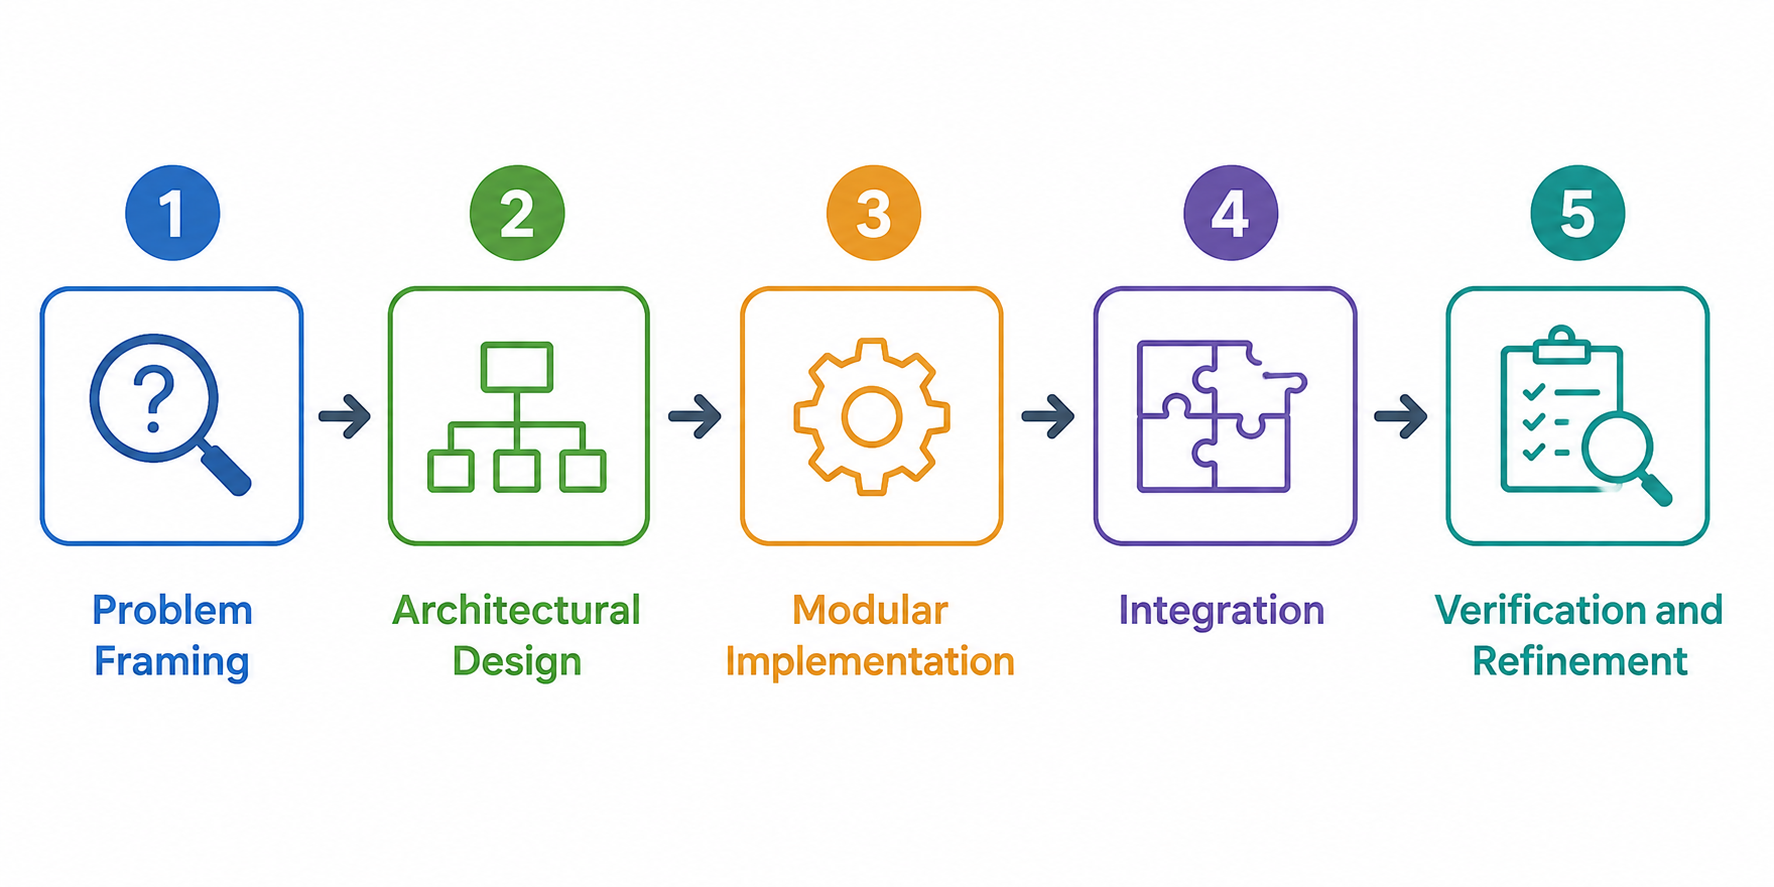
\includegraphics[
        width=0.85\textwidth,
        height=6cm,
        keepaspectratio
    ]{figures/research_phases.png}
    \caption{Research Design Phases}
    \label{fig:research-phases}
\end{figure}

The five phases shown in Figure~\ref{fig:research-phases} provide a structured path from problem identification to verification and refinement. Each phase contributes to the systematic development and evaluation of the proposed
crowd counting methodology.

% ==================================================
% PHASES OF RESEARCH DESIGN
% ==================================================

\begin{longtable}{|p{0.13\textwidth}|p{0.50\textwidth}|p{0.29\textwidth}|}

\caption{Phases of the Research Design}
\label{tab:research-design}\\

\hline
\textbf{Phase} & \textbf{Description} & \textbf{Primary Artifact(s)} \\
\hline
\endfirsthead

\hline
\textbf{Phase} & \textbf{Description} & \textbf{Primary Artifact(s)} \\
\hline
\endhead

\hline
\multicolumn{3}{r}{\textit{Continued on next page}} \\
\endfoot

\hline
\endlastfoot

Problem Framing &
Identify the limitations and trade offs between detection based approaches for relatively sparse crowds and regression based approaches for dense crowds, and establish the motivation for a hybrid counting framework. &
Problem statement, research objectives, and identified research gap \\
\hline

Architectural Design &
Decompose the proposed system into independent and sequential processing stages with clearly defined inputs, outputs, and responsibilities. &
System architecture and pipeline block diagram \\
\hline

Modular Implementation & Implement the individual processing stages as independent computational components with clearly defined interfaces and configurable parameters. & Modular system components and centralized configuration structure \\

\hline

Integration & Integrate the individual components into a unified processing pipeline capable of handling the intended visual input modalities. & Integrated computational pipeline and execution framework \\

\hline

Verification and Refinement & Execute the integrated system on representative image and video samples, examine intermediate outputs and computational performance, identify errors or inconsistencies, and refine relevant parameters and processing strategies. & Intermediate outputs, performance logs, experimental observations, and refined configurations \\

\hline
\end{longtable}

This design is deliberately experimental rather than purely descriptive. The pipeline exposes toggleable backends, such as YOLO versus Haar-cascade detection and classical versus neural density estimation, so that alternative configurations can be compared under identical inputs. This enables controlled, repeatable experiments rather than evaluation of a single fixed implementation.

\section{Research Approach}

An experimental research approach is adopted. Unlike a case study, which would examine one deployment in depth, or a survey, which would gather opinions or questionnaire data, this study manipulates system variables input modality, detection backend, density estimation backend, and decision thresholds and observes their effect on the dependent variables of interest: the estimated crowd count and its consistency across scene types. This is consistent with a quantitative, comparative experimental approach commonly used in 
computer vision systems research.

% ==================================================
% Independent and Dependent Variables
% ==================================================
\subsection{Independent and Dependent Variables}

Table~\ref{tab:experimental-variables} summarizes the independent and
dependent variables considered in the experimental evaluation.

\begin{longtable}{|p{0.18\textwidth}|p{0.30\textwidth}|p{0.42\textwidth}|}
\caption{Independent and Dependent Variables}
\label{tab:experimental-variables}\\
\hline

\textbf{Variable Type} &
\textbf{Variable} &
\textbf{Levels / Conditions} \\

\hline
\endfirsthead

\hline

\textbf{Variable Type} &
\textbf{Variable} &
\textbf{Levels / Conditions} \\

\hline
\endhead

\hline
\multicolumn{3}{r}{\textit{Continued on next page}}\\
\endfoot

\hline
\endlastfoot

Independent &
Detection Approach &
YOLO-based head detection and Haar-cascade-based head detection \\

\hline

Independent &
Density-Estimation Approach &
Classical density estimation and neural-network-based density estimation \\

\hline

Independent &
Scene-Density Decision &
Different threshold conditions for distinguishing relatively sparse and
relatively dense scenes \\

\hline

Independent &
Fusion Strategy &
Different weighting and decision strategies for combining detection-based
and density-based estimates \\

\hline

Independent &
Input Modality &
Single images and sampled video frames \\

\hline

Dependent &
Estimated Crowd Count &
Number of passengers estimated by the counting methodology \\

\hline

Dependent &
Scene Classification &
Classification of the input scene as relatively sparse or relatively dense \\

\hline

Dependent &
Counting Consistency &
Consistency of estimated passenger counts across consecutive video frames \\

\hline

Dependent &
Computational Performance &
Processing time required to generate the passenger-count estimate \\

\hline

\end{longtable}

The independent variables are systematically varied to examine their influence
on the dependent variables. Where appropriate, one experimental condition is
changed while the remaining conditions are kept constant. This allows the
effect of individual methodological components to be evaluated and supports
controlled comparison between alternative configurations.

% ==================================================
% 3.2.2 Justification
% ==================================================
\subsection{Justification}

The experimental approach is justified by the following considerations:

\begin{itemize}
    \item \textbf{Build-then-measure suitability:} 
    The research question---whether a hybrid sparse/dense approach can 
    outperform either approach alone across varying crowd densities---is 
    inherently a comparative, empirical question. It is therefore best 
    answered by implementing both approaches and measuring their outcomes, 
    rather than relying on case narratives or survey opinions.

    \item \textbf{Reproducibility:} 
    Deterministic, configuration-driven modules allow repeated trials under 
    identical settings, supporting the internal-validity requirements of 
    experimental research.

    \item \textbf{Scalability of evaluation:} 
    The same pipeline runs on both single images and video streams, enabling 
    experiments at multiple temporal scales, including single-frame accuracy 
    and video-level aggregate or unique-count behaviour.
\end{itemize}

% ==================================================
% 3.3 Data Collection Methods
% ==================================================
\section{Data Collection Methods}

Data collection in this study is based on two visual input modalities:
single static images and video sequences. Static images are directly used as
individual observations, while video data are sampled into representative
frames for subsequent analysis. This approach allows the proposed
crowd-counting methodology to be evaluated using both individual images and
temporally continuous visual data.

% ==================================================
% 3.3.1 Image and Video Acquisition
% ==================================================
\subsection{Image and Video Acquisition}

For image-based analysis, a single RGB image is used as the input to the
proposed processing pipeline. The image represents a particular scene and
provides the visual information required for passenger or crowd detection
and counting.

% ==================================================
% Data Collection INFOGRAPHIC
% ==================================================
\begin{figure}[htbp]
    \centering
    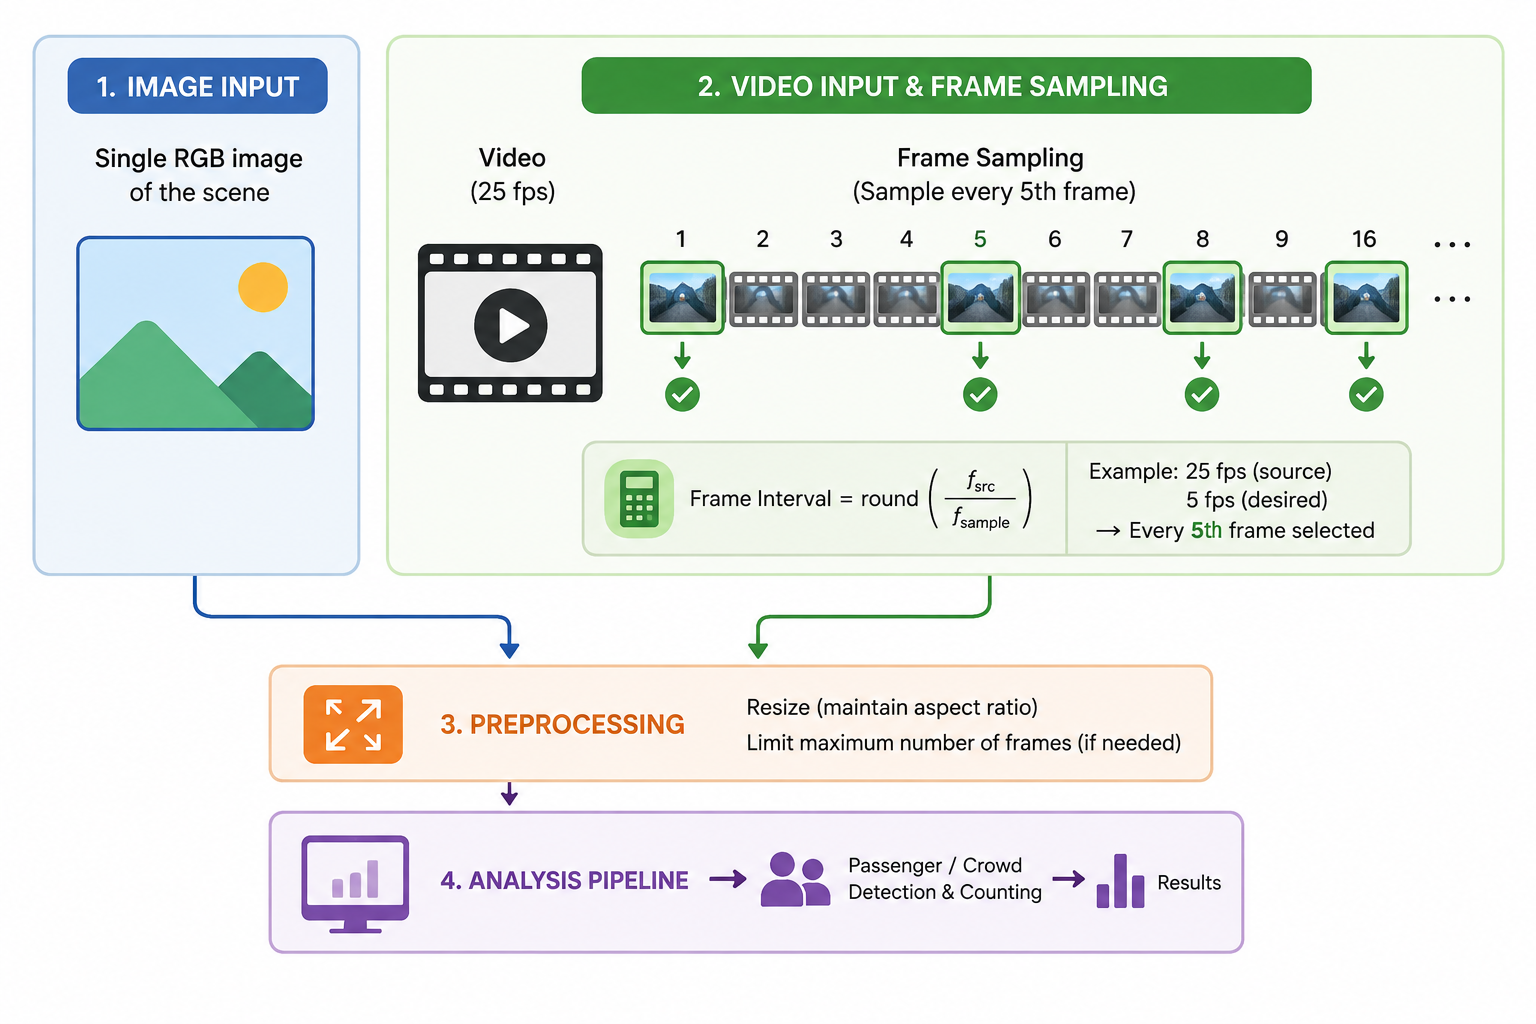
\includegraphics[
        width=0.95\textwidth,
        height=6cm,
        keepaspectratio
    ]{figures/image_and_video_acquisition.png}
    \caption{Image and Video Acquisition}
    \label{fig:image-and-video-acquisition}
\end{figure}

For video-based analysis, frames are systematically sampled from the video
sequence rather than processing every available frame. Temporal sampling is
used to reduce redundant observations and computational requirements while
retaining representative information from the video. The sampling interval
is determined according to the source frame rate and the desired sampling
rate.

The frame sampling interval is calculated as:

\begin{equation}
    \text{Frame Interval}
    =
    \operatorname{round}
    \left(
    \frac{f_{\mathrm{src}}}{f_{\mathrm{sample}}}
    \right)
\label{eq:frame-interval}
\end{equation}

where $f_{\mathrm{src}}$ represents the native frame rate of the source
video and $f_{\mathrm{sample}}$ represents the desired sampling rate.

For example, when a video has a native frame rate of 25 frames per second
and the desired sampling rate is 5 frames per second, approximately every
fifth frame is selected for analysis. This reduces the number of frames
requiring processing while maintaining temporal coverage of the video.

Before analysis, the selected frames may be resized while preserving their
original aspect ratio. A maximum number of frames may also be specified
when bounded-duration experiments are required. These procedures provide
consistent input dimensions and manageable computational requirements
during experimental evaluation.


% ==================================================
% 3.3.2 Data Sources and Domain
% ==================================================
\subsection{Data Sources and Domain}

The proposed system is designed primarily for passenger and crowd-counting applications in public-transport and public-space environments specially in bus interiors. The methodology is not restricted to a single type of visual source.
Potential input sources include surveillance-camera footage, elevated-camera
footage, photographs, and other RGB image or video sources containing
crowded scenes. This source flexibility allows the proposed approach to be
evaluated under different scene layouts, viewing angles, illumination
conditions, and crowd-density levels.

For the experimental evaluation, the selected dataset or field-collected
visual samples should contain representative scenes covering relatively
sparse, moderate, and dense crowd conditions. The selected data should also
provide sufficient variation in terms of passenger arrangement, occlusion,
viewpoint, and scene composition to support a meaningful evaluation of the
proposed methodology.

% ==================================================
% 3.3.3 Pre-trained Model Assets
% ==================================================
\subsection{Pre-trained Model Assets}

The proposed methodology employs pre-trained model components to perform
detection and density-estimation tasks. These components provide the
underlying feature extraction, object detection, and density-estimation
capabilities required by the proposed crowd-counting framework.

\begin{longtable}{|p{0.25\textwidth}|p{0.30\textwidth}|p{0.35\textwidth}|}
\caption{Pre-trained Model Assets}
\label{tab:pretrained-assets}\\
\hline

\textbf{Asset} &
\textbf{Role} &
\textbf{Description} \\

\hline
\endfirsthead

\hline

\textbf{Asset} &
\textbf{Role} &
\textbf{Description} \\

\hline
\endhead

\hline
\multicolumn{3}{r}{\textit{Continued on next page}}\\
\endfoot

\hline
\endlastfoot

YOLOv8-nano &
Sparse crowd detection &
A lightweight object-detection model used to identify person or head
regions in relatively sparse scenes. \\

\hline

Haar Cascade &
Alternative sparse detection &
A lightweight classical detection method that can be used as an
alternative detection approach for relatively sparse scenes. \\

\hline

Four-Column CNN &
Dense crowd estimation &
A neural-network-based density-regression model used to estimate crowd
density in relatively dense scenes where individual detections may be
affected by significant occlusion. \\

\hline

\end{longtable}


% ==================================================
% 3.3.4 Ground-Truth Collection for Evaluation
% ==================================================
% \subsection{Ground-Truth Collection for Evaluation}

% Ground-truth annotations are required to quantitatively evaluate the
% accuracy of the proposed crowd-counting methodology. A representative
% sample of images or video frames is selected from the collected data,
% ensuring coverage of relatively sparse, moderate, and dense crowd
% conditions.

% For each selected frame, the number of visible passenger heads is manually
% annotated to establish the reference crowd count. To improve annotation
% reliability, at least two independent human annotators are assigned to
% count the visible heads in each selected frame. Their annotations are then
% compared to identify disagreements.

% When disagreements occur, the final ground-truth count is established
% through consensus between the annotators or by an additional adjudication
% process. The resulting agreed count is treated as the reference ground
% truth for subsequent accuracy and error analysis.

% The collected ground-truth annotations are subsequently compared with the
% counts generated by the proposed methodology. This comparison provides the
% basis for calculating quantitative evaluation measures such as counting
% error, mean absolute error (MAE), root mean squared error (RMSE), and
% accuracy-related measures described in the subsequent data-analysis
% section.

% ==================================================
% 3.4 Data Analysis Techniques
% ==================================================
\section{Data Analysis Techniques}

Data analysis in this study is performed at three complementary levels:
image-level analysis used to condition and enhance the input, algorithmic and
statistical analysis used to convert detections and density information into
crowd counts, and system-level analysis used to evaluate computational
performance and counting behaviour. These analytical procedures collectively
support the processing, interpretation, and evaluation of the proposed
crowd-counting methodology.


% ==================================================
% 3.4.1 Image Pre-processing Analysis
% ==================================================
\subsection{Image Pre-processing Analysis}

Image pre-processing is performed to improve the visual quality of input
frames before detection and density estimation. Contrast-Limited Adaptive
Histogram Equalization (CLAHE) is applied to the luminance component of the
image after conversion to the CIELAB colour space. This is followed by an
optional Gaussian smoothing operation.

The enhanced luminance component is expressed as:

\begin{equation}
L' = \operatorname{CLAHE}
\left(
L;\,\text{clipLimit}=2.0,\,
\text{tileGridSize}=8\times8
\right)
\label{eq:clahe}
\end{equation}

where $L$ represents the luminance channel of the CIELAB image and $L'$
represents the contrast-enhanced luminance channel.

The enhanced image is then reconstructed using the original chromatic
components and optionally smoothed using a Gaussian filter:

\begin{equation}
I_{\mathrm{out}} =
\operatorname{GaussianBlur}
\left(
\operatorname{merge}(L',a,b);
\text{kernel}=3\times3
\right)
\label{eq:gaussian}
\end{equation}

CLAHE improves local contrast in scenes containing uneven illumination,
shadows, or backlighting. Gaussian smoothing further reduces high-frequency
noise while preserving the major structural information required for
subsequent detection and density-estimation stages.


% ==================================================
% 3.4.2 Detection-Level Analysis
% ==================================================
\subsection{Detection-Level Analysis: Overlap and Suppression}
\label{sec:nms}

Spatial reasoning during detection and counting relies on the
Intersection-over-Union (IoU) measure. IoU quantifies the degree of spatial
overlap between two axis-aligned bounding boxes $A$ and $B$ and is defined as:

\begin{equation}
\operatorname{IoU}(A,B)
=
\frac{|A\cap B|}
{|A\cup B|}
\label{eq:iou}
\end{equation}

where $|A\cap B|$ represents the area of intersection between the two
bounding boxes and $|A\cup B|$ represents their union area.

When multiple detections correspond to the same person or highly overlapping
regions, redundant detections are removed using Non-Maximum Suppression
(NMS). The detection with the highest confidence within an overlapping group
is retained while lower-confidence redundant detections are suppressed.

The resulting sparse count can therefore be expressed as:

\begin{equation}
C_{\mathrm{sparse}}
=
\left|
\left\{
d\in D:
d\text{ survives NMS}
\left(\tau_{\mathrm{IoU}}=0.35\right)
\right\}
\right|
\label{eq:sparse-count}
\end{equation}

where $D$ denotes the initial set of detections and
$\tau_{\mathrm{IoU}}$ represents the IoU threshold used for suppression.


% ==================================================
% 3.4.3 Scene-Density Analysis
% ==================================================
\subsection{Scene-Density Analysis: Sparse and Dense Classification}
\label{sec:density-analysis}

The input scene is classified as either relatively sparse or relatively
dense using statistical characteristics derived from the detected regions.
Two primary statistics are considered: normalized detection density and
pairwise overlap ratio.

The normalized detection density is calculated as:

\begin{equation}
\rho =
\frac{N}
{hw/1000}
\label{eq:detection-density}
\end{equation}

where $N$ is the number of detected regions, while $h$ and $w$ represent the
height and width of the input frame in pixels, respectively. The resulting
value represents the number of detections per $1000$ pixels$^2$.

The pairwise overlap ratio is calculated by considering the set of all
unordered pairs of detections:

\begin{equation}
\omega =
\frac{
\left|
\left\{
(a,b)\in P:
\operatorname{IoU}(a,b)>0
\right\}
\right|
}
{|P|}
\label{eq:overlap-ratio}
\end{equation}

where $P$ denotes the set of all unordered pairs of detected regions.

The scene is classified according to the following decision rule:

\begin{equation}
\text{Scene} =
\begin{cases}
\text{Dense}, &
N\geq N_{\min}
\quad\text{and}\quad
(\rho\geq\tau_{\rho}
\;\text{or}\;
\omega\geq\tau_{\omega})
\\[6pt]
\text{Sparse}, & \text{otherwise}
\end{cases}
\label{eq:scene-classification}
\end{equation}

where $N_{\min}$ represents the minimum number of detections required for
dense-scene evaluation, $\tau_{\rho}$ represents the detection-density
threshold, and $\tau_{\omega}$ represents the overlap-ratio threshold.

For the experimental configuration, the default values are:

\begin{equation}
N_{\min}=15,\qquad
\tau_{\rho}=0.35,\qquad
\tau_{\omega}=0.15
\label{eq:density-thresholds}
\end{equation}

The resulting scene classification determines whether the sparse or dense
counting approach receives greater importance during the subsequent fusion
stage.


% ==================================================
% 3.4.4 Dense-Branch Signal Analysis
% ==================================================
\subsection{Dense-Branch Signal Analysis}

The dense-counting branch uses density information to estimate the number of
people in scenes where individual detections may be unreliable because of
occlusion, small object size, or high crowd density.

For the classical density-estimation approach, detected regions are
represented as point masses at their corresponding centroids. These points
are spatially smoothed using a Gaussian kernel to generate a continuous
density representation. An edge-based correction component may additionally
be incorporated to account for visually dense regions that are not directly
detected.

For the neural density-estimation approach, the input image is processed by
a neural density-regression model to produce a predicted density map. The
estimated crowd count is obtained by integrating, or summing, the values of
the predicted density map:

\begin{equation}
C_{\mathrm{dense}}
=
\sum_{x=1}^{W}
\sum_{y=1}^{H}
D(x,y)
\label{eq:dense-count}
\end{equation}

where $D(x,y)$ represents the estimated density at spatial location
$(x,y)$, while $W$ and $H$ represent the width and height of the density
map, respectively.


% ==================================================
% 3.4.5 Fusion and Disagreement Analysis
% ==================================================
\subsection{Fusion and Disagreement Analysis}

The sparse and dense branches produce complementary estimates of the crowd
count. The sparse branch provides explicit individual detections, whereas
the dense branch provides an aggregate estimate based on the spatial
distribution of crowd information.

The two estimates are combined using a weighted fusion strategy. The
relative contribution of each branch is determined according to the
characteristics of the input scene. In addition, a disagreement criterion
can be used to identify cases in which the two estimates differ
substantially.

The general form of the fused estimate is:

\begin{equation}
C_{\mathrm{fused}}
=
w_s C_{\mathrm{sparse}}
+
w_d C_{\mathrm{dense}}
\label{eq:fused-count}
\end{equation}

subject to:

\begin{equation}
w_s+w_d=1
\label{eq:fusion-weights}
\end{equation}

where $C_{\mathrm{sparse}}$ and $C_{\mathrm{dense}}$ represent the
sparse- and dense-branch estimates, respectively, while $w_s$ and $w_d$
represent their corresponding fusion weights.

This fusion mechanism can be interpreted as a simple multi-source
estimation strategy in which complementary counting estimates are combined
to improve robustness across different crowd-density conditions.


% ==================================================
% 3.4.6 Runtime and Performance Analysis
% ==================================================
\subsection{Runtime and Performance Analysis}

System-level analysis considers the computational performance of the
proposed methodology. The processing time required by the major stages,
including pre-processing, detection, and density estimation, is recorded
for each processed frame.

For a video containing $T$ sampled frames, the mean fused crowd count is
calculated as:

\begin{equation}
\overline{C}
=
\frac{1}{T}
\sum_{t=1}^{T}
C_{\mathrm{fused},t}
\label{eq:mean-fused-count}
\end{equation}

where $C_{\mathrm{fused},t}$ denotes the fused crowd count for frame $t$.

In addition to the mean count, the maximum estimated count across the
sampled frames can be used to characterize the variation in observed crowd
levels throughout the video. Processing latency is also considered as an
important system-level measure because practical passenger-counting
applications require timely analysis of incoming visual data.


% ==================================================
% 3.4.7 Accuracy Evaluation Metrics
% ==================================================
\subsection{Accuracy Evaluation Metrics}

To quantitatively evaluate the accuracy of the proposed crowd-counting
methodology, the predicted counts are compared against the ground-truth
counts. Mean Absolute Error (MAE) and Root Mean
Squared Error (RMSE) are used as the primary counting-error metrics.

For $M$ evaluation frames, where $\hat{c}_i$ represents the predicted count
and $c_i$ represents the corresponding ground-truth count, MAE is calculated
as:

\begin{equation}
\operatorname{MAE}
=
\frac{1}{M}
\sum_{i=1}^{M}
\left|
\hat{c}_i-c_i
\right|
\label{eq:mae}
\end{equation}

MAE represents the average absolute difference between the predicted and
ground-truth counts. A lower MAE indicates better counting accuracy.

RMSE is calculated as:

\begin{equation}
\operatorname{RMSE}
=
\sqrt{
\frac{1}{M}
\sum_{i=1}^{M}
\left(
\hat{c}_i-c_i
\right)^2
}
\label{eq:rmse}
\end{equation}

RMSE assigns greater importance to larger counting errors because the
individual errors are squared before averaging. Therefore, it is useful for
identifying cases in which the proposed methodology produces substantial
counting deviations.

These metrics enable quantitative comparison among the sparse-only,
dense-only, and fused counting configurations. The results can subsequently
be analyzed across different crowd-density conditions to determine the
accuracy, robustness, and consistency of the proposed methodology.

% ==================================================
% Proposed Algorithm / Model / Techniques
% ==================================================
\section{Proposed Algorithm}

This section presents the proposed hybrid sparse/dense crowd-counting
methodology. The overall framework combines detection-based counting for
relatively sparse scenes with density-estimation-based counting for relatively dense scenes. The two complementary estimates are subsequently combined through a scene-aware fusion strategy. 

% For video input, a multi-object tracking mechanism is additionally considered to estimate the number of unique individuals across consecutive frames.

The overall processing sequence of the proposed methodology is illustrated
in Figure~\ref{fig:hybrid-architecture}.

% ==================================================
% Figure 3.1
% ==================================================
\begin{figure}[htbp]
    \centering
    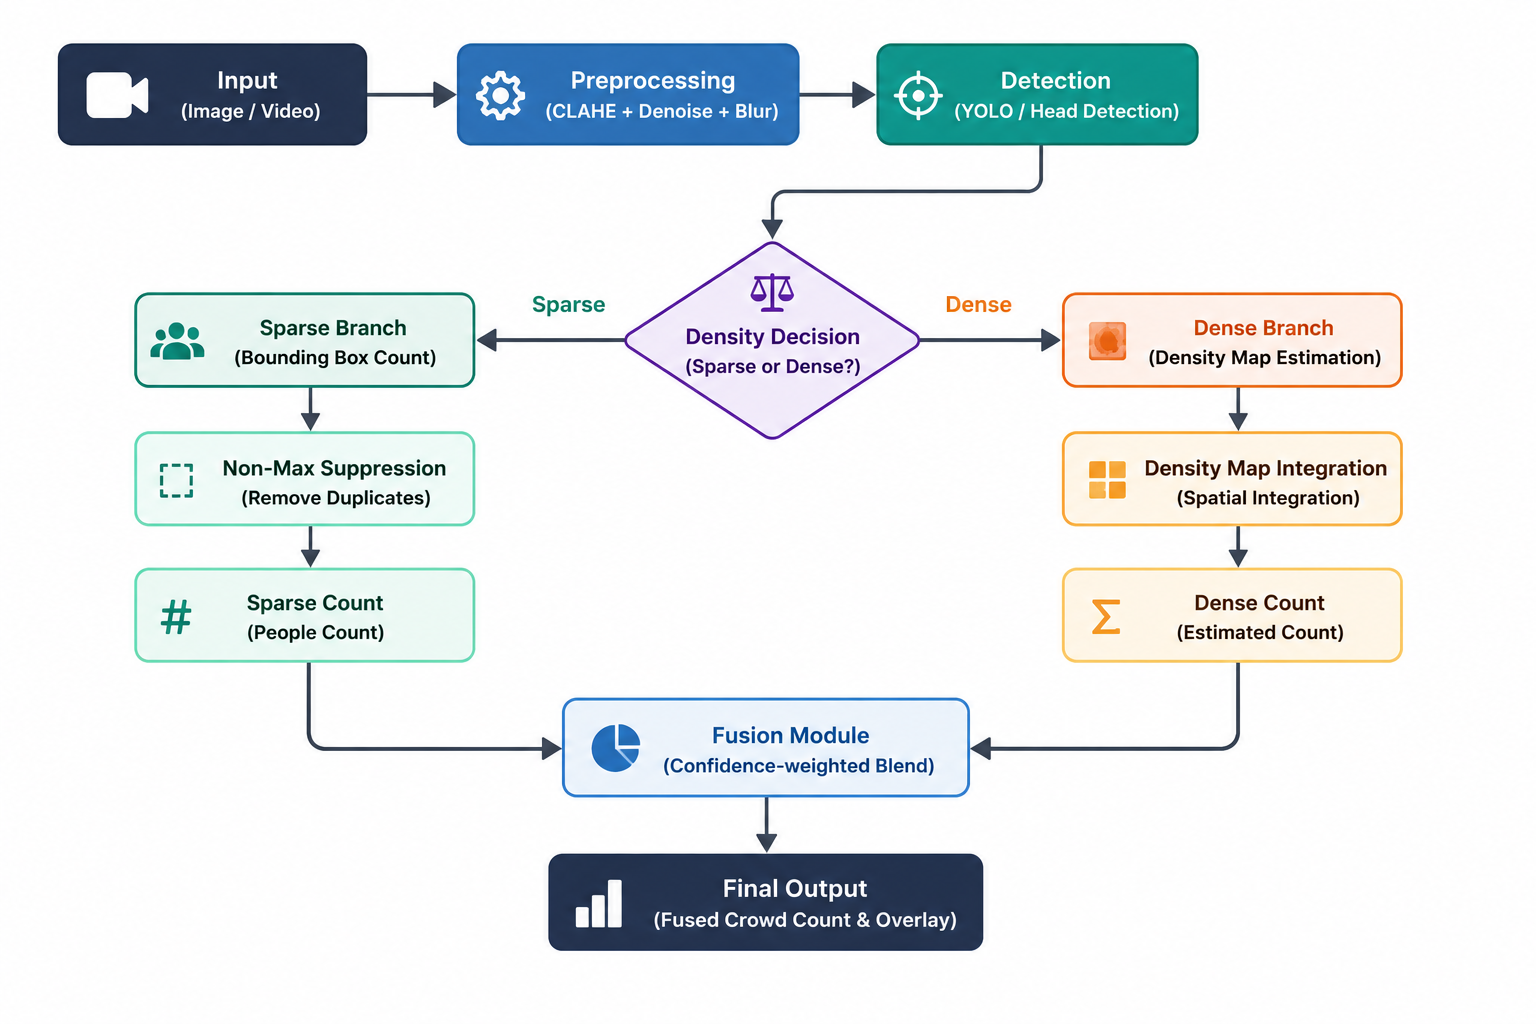
\includegraphics[
        width=0.90\textwidth
    ]{figures/hybrid_architecture.png}
    \caption{Hybrid Sparse/Dense Crowd Counting Architecture}
    \label{fig:hybrid-architecture}
\end{figure}


% ==================================================
% 3.5.1 Design Rationale
% ==================================================
\subsection{Design Rationale}

The proposed hybrid methodology is motivated by the complementary strengths
and limitations of detection-based and density-estimation-based crowd
counting approaches.

\begin{itemize}

\item \textbf{Detection-based counting:}
Individual head or person detections provide precise and interpretable
counts in relatively sparse and moderately crowded scenes. However, the
performance of individual detection may decrease substantially in highly
crowded scenes because of occlusion, small object size, and overlapping
detections.

\item \textbf{Density-based counting:}
Density-map estimation is more suitable for highly crowded scenes where
individual people cannot be reliably separated. However, density regression
may provide less precise individual counts in sparse scenes where explicit
detections can be obtained reliably.

\item \textbf{Hybrid counting:}
The proposed methodology combines both approaches and uses scene-density
information to determine the relative importance of the two estimates. This
allows the system to exploit the strengths of each approach while reducing
the limitations associated with relying exclusively on either detection or
density estimation.

\end{itemize}


% ==================================================
% 3.5.2 Sparse Branch
% ==================================================
\subsection{Sparse Branch: Head and Person Detection}

The sparse branch identifies individual people or head regions and uses the
resulting detections to estimate the crowd count. Two alternative detection
approaches are considered: a YOLO-based object detector and a classical
Haar-cascade detector.

The YOLO-based approach performs single-stage object detection and retains
detections corresponding to the person category whose confidence exceeds
the predefined confidence threshold. The detected bounding boxes are then
subjected to Non-Maximum Suppression (NMS), as described in \cref{sec:nms}, to remove redundant overlapping detections.

The alternative approach uses a classical Haar-cascade detector. This
lightweight detection method provides an additional option for scenes in
which a computationally simpler detection mechanism is desirable.

The detections that remain after the suppression process are used to
calculate the sparse crowd count:

\begin{equation}
C_{\mathrm{sparse}}
=
\left|D_{\mathrm{retained}}\right|
\label{eq:proposed-sparse-count}
\end{equation}

where $D_{\mathrm{retained}}$ represents the set of detections remaining
after confidence filtering and Non-Maximum Suppression.

The detected regions can also be visualized using bounding boxes and
confidence values. Such visualization provides qualitative evidence for
examining detection behaviour and identifying common failure cases such as
missed detections, false positives, and overlapping detections.


% ==================================================
% 3.5.3 Density Decision Module
% ==================================================
\subsection{Density Decision Module}

The density decision module determines whether the input scene should be
treated as relatively sparse or relatively dense. The decision is based on
the statistical characteristics of the initial detections, particularly
normalized detection density and the degree of spatial overlap between
detected regions.

The decision procedure described in \cref{sec:density-analysis} produces one of two scene
labels:

\begin{equation}
S =
\begin{cases}
\text{Sparse}, & \text{if the scene satisfies the sparse condition},\\
\text{Dense}, & \text{if the scene satisfies the dense condition}.
\end{cases}
\label{eq:scene-label}
\end{equation}

The resulting scene label is subsequently supplied to the fusion stage.
The label determines which counting branch is considered the primary source
of information for the final estimate.


% ==================================================
% 3.5.4 Dense Branch
% ==================================================
\subsection{Dense Branch: Density-Map Estimation}

The dense branch estimates the crowd count from a spatial density
representation rather than relying exclusively on individual detections.
Two density-estimation approaches are considered: a classical Gaussian
kernel-based method with edge correction and a neural-network-based density
regression method.


% ==================================================
% Classical Density Estimation
% ==================================================
\subsubsection{Classical Density Estimation}

In the classical approach, the centroids of the detected regions are
represented as point masses on a spatial grid. These point masses are then
smoothed using an isotropic Gaussian kernel with standard deviation
$\sigma$.

The detection-derived density map is expressed as:

\begin{equation}
D_{\mathrm{det}}(x,y)
=
G_{\sigma}(x,y)
*
\sum_{k}
\delta(x-x_k,y-y_k)
\label{eq:detection-density-map}
\end{equation}

where $G_{\sigma}$ represents the Gaussian kernel, $\delta$ represents the
Dirac delta function, and $(x_k,y_k)$ denotes the centroid of the $k$-th
detected region.

To compensate for visually dense regions that may contain undetected
individuals, an edge-based correction term is incorporated. The correction
is derived from the edge structure of the input image and is scaled so that
its contribution remains bounded relative to the detection-derived density.

The edge correction can be expressed as:

\begin{equation}
E'(x,y)
=
E(x,y)
\left[
\frac{0.15\,M_{\mathrm{det}}}
{\sum_{x,y}E(x,y)}
\right]
\label{eq:edge-correction}
\end{equation}

where $E(x,y)$ represents the smoothed edge-derived density and
$M_{\mathrm{det}}$ represents the total mass of the detection-derived
density map:

\begin{equation}
M_{\mathrm{det}}
=
\sum_{x,y}
D_{\mathrm{det}}(x,y)
\label{eq:detection-mass}
\end{equation}

The final classical density map is therefore:

\begin{equation}
D(x,y)
=
D_{\mathrm{det}}(x,y)
+
E'(x,y)
\label{eq:classical-density-map}
\end{equation}

and the corresponding dense crowd estimate is obtained by integrating the
density map:

\begin{equation}
C_{\mathrm{dense}}
=
\sum_{x,y}D(x,y)
\label{eq:classical-dense-count}
\end{equation}

The bounded correction factor limits the influence of image texture and
reduces the risk of excessive counting caused by noisy or irrelevant edge
structures.


% ==================================================
% Neural Density Estimation
% ==================================================
\subsubsection{Neural Density Estimation: Four-Column MDNN}

The neural density-estimation branch uses a Four-Column Multi-Column
Density Neural Network (MDNN). The architecture is designed to capture
visual information at multiple spatial scales, which is important for crowd
scenes in which the apparent size of heads varies according to their
distance from the camera.

The architecture consists of four parallel convolutional columns. Each
column uses a different sequence of convolutional kernel sizes and is
designed to capture information at a particular spatial scale.

\begin{table}[htbp]
\centering
\caption{Column-Wise Configuration of the Four-Column MDNN}
\label{tab:mdnn-columns}
\renewcommand{\arraystretch}{1.2}

\begin{tabularx}{\textwidth}{c c c c X}
\hline
\textbf{Column} &
\textbf{Receptive Field} &
\textbf{Kernel Progression} &
\textbf{Output Channels} &
\textbf{Design Intent} \\
\hline

1 & Very large & $11 \rightarrow 9 \rightarrow 7$ & 64 &
Capture very close and relatively large heads \\

\hline

2 & Large & $9 \rightarrow 7 \rightarrow 5$ & 64 &
Capture moderately close heads \\

\hline

3 & Medium & $7 \rightarrow 5 \rightarrow 3$ & 80 &
Capture heads at intermediate distances \\

\hline

4 & Small & $5 \rightarrow 3 \rightarrow 3$ & 96 &
Capture small, distant, and densely distributed heads \\

\hline
\end{tabularx}
\end{table}


Each column applies convolutional, batch-normalization, activation, and
pooling operations to progressively extract features at different spatial
scales. The resulting feature maps are concatenated along the channel
dimension.

If $f_1(I)$, $f_2(I)$, $f_3(I)$, and $f_4(I)$ represent the feature maps
generated by the four columns for input image $I$, their concatenation is
given by:

\begin{equation}
F(I)
=
\operatorname{Concat}
\left[
f_1(I),
f_2(I),
f_3(I),
f_4(I)
\right]
\label{eq:mdnn-concat}
\end{equation}

The four feature-map groups provide a total of

\begin{equation}
64+64+80+96=304
\label{eq:mdnn-channels}
\end{equation}

feature channels.

The concatenated feature representation is then passed through a
convolutional fusion head to generate a single-channel density map:

\begin{equation}
D(x,y)
=
\operatorname{ReLU}
\left(
W_2
\cdot
\operatorname{ReLU}
\left(
W_1\cdot F(I)
\right)
\right)
\label{eq:mdnn-density}
\end{equation}

where $W_1$ represents the first fusion layer and $W_2$ represents the
second fusion layer. The predicted dense count is calculated by summing the
values of the resulting density map:

\begin{equation}
C_{\mathrm{dense}}
=
\sum_{x,y}D(x,y)
\label{eq:mdnn-count}
\end{equation}

The multi-column structure allows the model to process visual features
associated with different apparent head sizes within the same image.


% ==================================================
% Figure 3.2
% ==================================================
\begin{figure}[htbp]
    \centering
    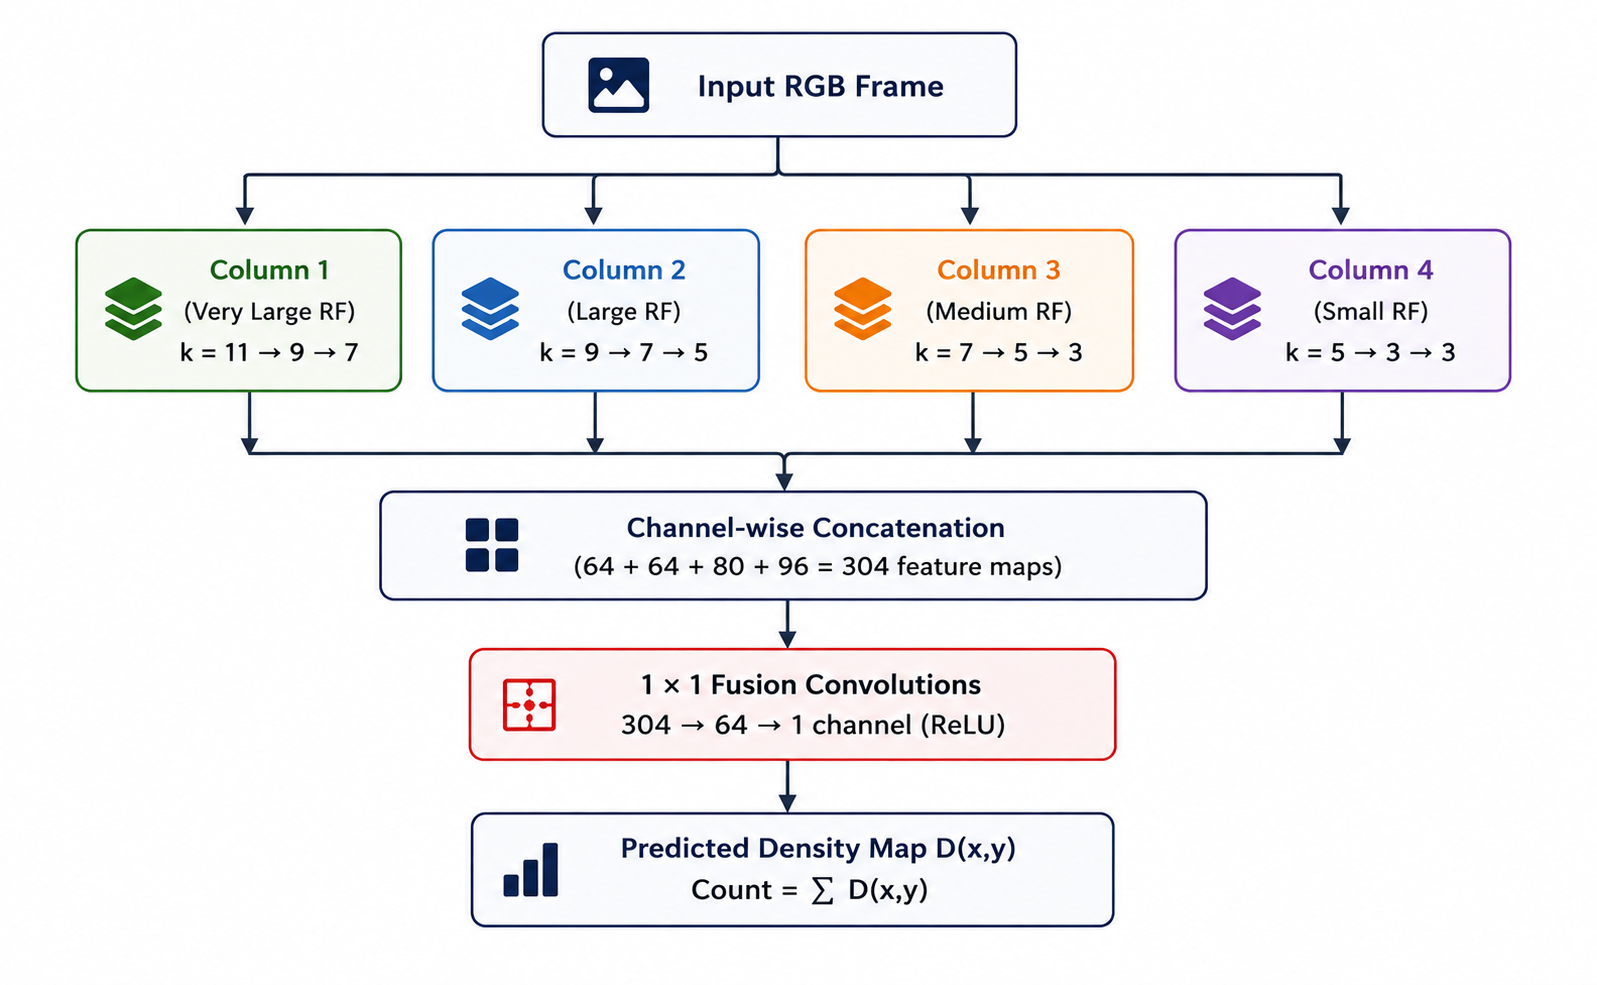
\includegraphics[
        width=0.85\textwidth
    ]{figures/four_column_mdnn.png}
    \caption{Four-Column Multi-Column Density Neural Network (MDNN)}
    \label{fig:mdnn-architecture}
\end{figure}


The Four-Column MDNN architecture shown in
Figure~\ref{fig:mdnn-architecture} provides multiple receptive-field
scales for extracting crowd-related features.


% ==================================================
% 3.5.5 Fusion Module
% ==================================================
\subsection{Fusion Module}

The fusion module combines the sparse and dense crowd estimates according
to the scene-density classification. The scene label determines which
estimate is treated as the primary estimate.

The primary and secondary estimates are defined as:

\begin{equation}
(C_{\mathrm{primary}},C_{\mathrm{secondary}})
=
\begin{cases}
(C_{\mathrm{sparse}},C_{\mathrm{dense}}),
& \text{if the scene is sparse},\\[4pt]
(C_{\mathrm{dense}},C_{\mathrm{sparse}}),
& \text{if the scene is dense}.
\end{cases}
\label{eq:primary-secondary}
\end{equation}

The relative disagreement between the two estimates is calculated as:

\begin{equation}
\Delta
=
\frac{
\left|
C_{\mathrm{primary}}
-
C_{\mathrm{secondary}}
\right|
}
{C_{\mathrm{primary}}}
\label{eq:disagreement}
\end{equation}

When the disagreement exceeds a predefined threshold, the primary estimate
is retained. Otherwise, the two estimates are combined using a weighted
average:

\begin{equation}
C_{\mathrm{fused}}
=
\begin{cases}
C_{\mathrm{primary}},
& \Delta > 0.5,\\[6pt]
\displaystyle
\frac{
w_1C_{\mathrm{primary}}
+
w_2C_{\mathrm{secondary}}
}
{w_1+w_2},
& \Delta \leq 0.5.
\end{cases}
\label{eq:fusion}
\end{equation}

where $w_1$ and $w_2$ represent the weights assigned to the primary and
secondary estimates, respectively.

The default configuration uses equal weights:

\begin{equation}
w_1=w_2=1
\label{eq:fusion-default-weights}
\end{equation}

The fusion strategy therefore has two principal behaviours. When the two
branches produce reasonably consistent estimates, their information is
combined through weighted averaging. When substantial disagreement occurs,
the estimate associated with the scene-appropriate branch is retained. This
reduces the influence of a potentially unreliable secondary estimate.


% ==================================================
% Figure 3.3
% ==================================================
\begin{figure}[htbp]
    \centering
    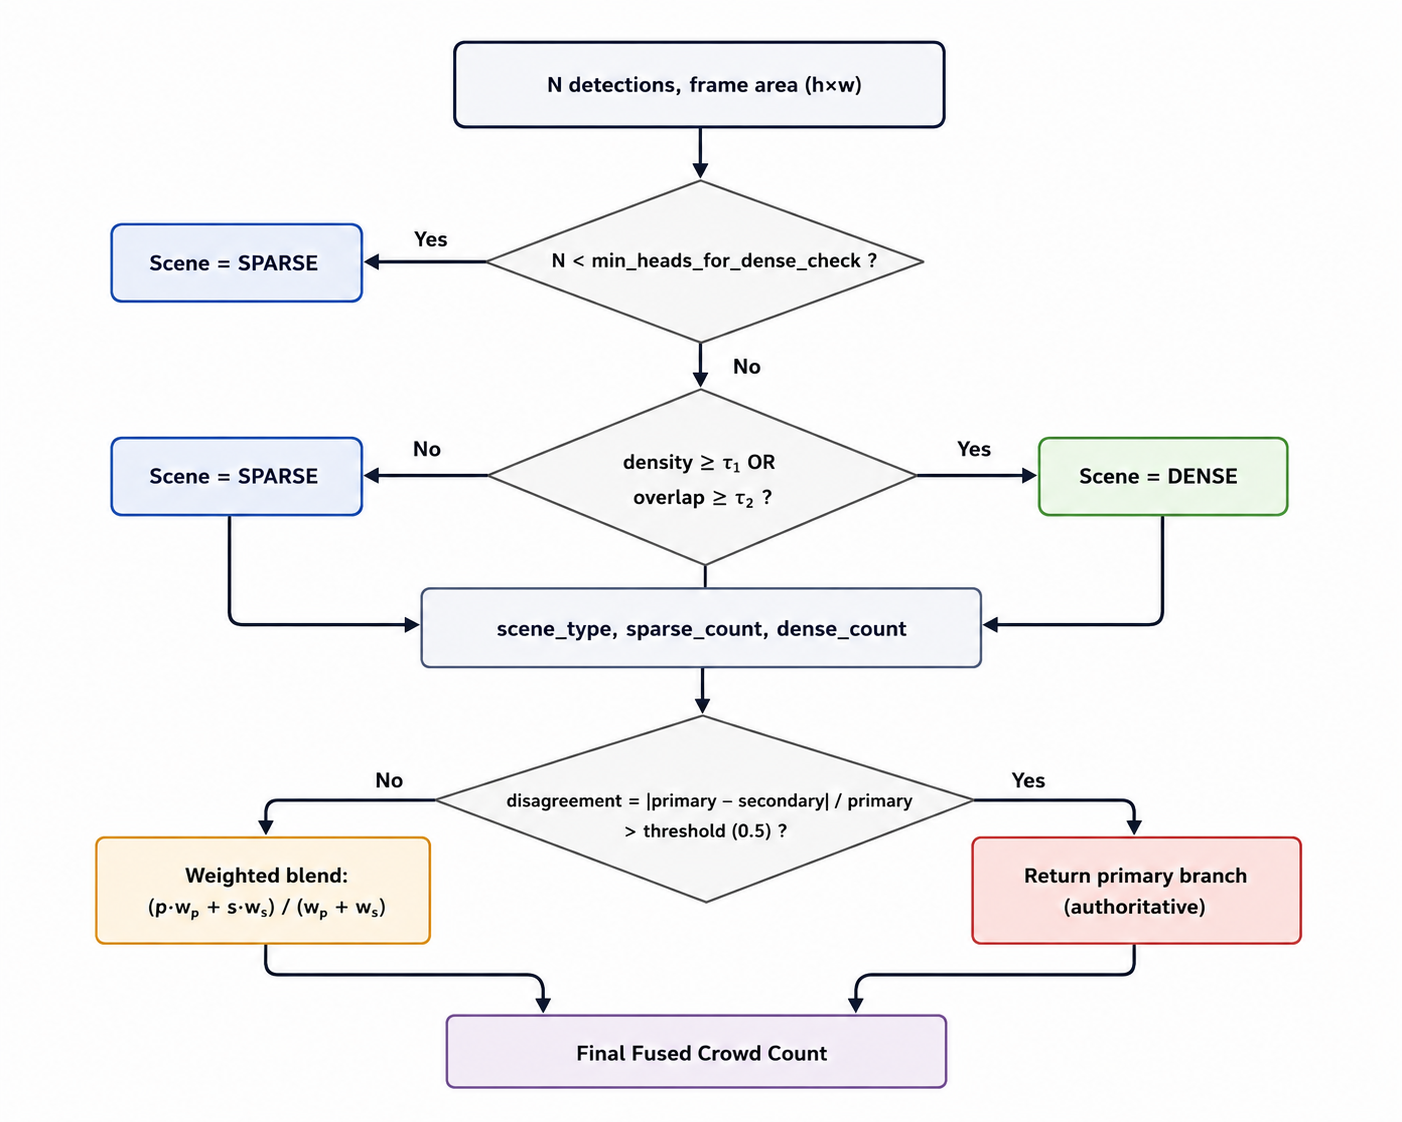
\includegraphics[
        width=0.80\textwidth
    ]{figures/fusion_decision_logic.png}
    \caption{Density Decision and Fusion Logic}
    \label{fig:fusion-logic}
\end{figure}


The overall density-decision and fusion process is illustrated in
Figure~\ref{fig:fusion-logic}.


% ==================================================
% 3.5.6 Multi-Object Tracking
% ==================================================
\subsection{Multi-Object Tracking: Video-Level Unique-Individual Count}

For video input, a multi-object tracking mechanism can be used to associate
individual detections across consecutive frames. This prevents the same
person, when visible across multiple frames, from being counted repeatedly
when estimating the number of unique individuals observed throughout the
video.

Track-to-detection association is formulated as a linear assignment
problem. The cost associated with assigning detection $j$ to track $i$ is
defined using the Intersection-over-Union measure:

\begin{equation}
\operatorname{cost}(i,j)
=
1-\operatorname{IoU}
\left(
\operatorname{track}_i,
\operatorname{detection}_j
\right)
\label{eq:tracking-cost}
\end{equation}

The Hungarian algorithm is used to obtain an optimal assignment between
existing tracks and current-frame detections. An assignment is accepted
only when the corresponding IoU exceeds a predefined matching threshold.

A track is considered confirmed after accumulating a minimum number of
consecutive successful matches. Conversely, a track is removed when it
remains unmatched for more than a predefined number of consecutive frames.

The track-status conditions can therefore be represented as:

\begin{equation}
\text{Track confirmed}
\iff
\text{hits}\geq 2
\label{eq:track-confirmed}
\end{equation}

and

\begin{equation}
\text{Track purged}
\iff
\text{missed}>8
\label{eq:track-purged}
\end{equation}

This mechanism allows short-term occlusions or missed detections to be
handled without immediately terminating an existing track. Consequently,
the same individual can be maintained as a single tracked entity across
multiple consecutive frames.

The unique-individual count can then be expressed as:

\begin{equation}
C_{\mathrm{unique}}
=
\left|
\left\{
t:
t\text{ is a confirmed track}
\right\}
\right|
\label{eq:unique-count}
\end{equation}

The tracking component is considered an extension of the frame-level
counting methodology for video-based analysis. Its primary purpose is to
improve temporal consistency and prevent repeated observations of the same
individual from being interpreted as separate passengers.


% ==================================================
% 3.5.7 End-to-End Pipeline Algorithm
% ==================================================
\subsection{End-to-End Pipeline Algorithm}

The complete per-frame algorithm for the proposed hybrid sparse/dense
crowd-counting framework is summarized in Algorithm~\ref{alg:hybrid-counting}.
For video input, the same frame-level procedure is repeated for each sampled
frame, while the tracking mechanism maintains the identities of detected
individuals across consecutive frames.

% --------------------------------------------------
% Algorithm 3.1
% --------------------------------------------------
\begin{algorithm}[htbp]
\caption{Hybrid Sparse/Dense Crowd Counting for a Single Frame}
\label{alg:hybrid-counting}

\begin{algorithmic}[1]

\Require Raw frame $I$ of dimensions $H \times W \times 3$
\Ensure $C_{\mathrm{sparse}}$, $C_{\mathrm{dense}}$,
$C_{\mathrm{fused}}$, and scene type $S$

\State $I' \gets \mathrm{Preprocess}(I)$
    \Comment{Contrast enhancement and smoothing}

\State $D \gets \mathrm{HeadDetector}(I')$
    \Comment{Head/person detection}

\State $S \gets \mathrm{DensityDecision}(D,H,W)$
    \Comment{Sparse or dense classification}

\State $(C_{\mathrm{sparse}},D_{\mathrm{kept}})
    \gets \mathrm{NMSCount}(D,0.35)$
    \Comment{Remove redundant detections}

\State $(M,C_{\mathrm{dense}})
    \gets \mathrm{DensityPredictor}(I',D)$
    \Comment{Density-map estimation}

\State $C_{\mathrm{fused}}
    \gets \mathrm{Fuse}(S,C_{\mathrm{sparse}},C_{\mathrm{dense}})$

\State \Return
$\{C_{\mathrm{sparse}},C_{\mathrm{dense}},
C_{\mathrm{fused}},S\}$

\end{algorithmic}
\end{algorithm}


% --------------------------------------------------
% Algorithm 3.2
% --------------------------------------------------

\begin{algorithm}[htbp]
\caption{Video-Level Extension of the Proposed Counting Method}
\label{alg:video-counting}

\begin{algorithmic}[1]

\Require Input video $V$ and sampling rate $f_{\mathrm{sample}}$
\Ensure Average count, maximum count, and unique-individual count

\For{each sampled frame $(i,t,I_i)$ from $V$}

    \State $R_i \gets \mathrm{HybridCounting}(I_i)$

    \State $T_i \gets \mathrm{TrackerUpdate}(D_i)$
        \Comment{IoU-based association}

    \State Store annotated frame and counting results

\EndFor

\State $C_{\mathrm{avg}}
    \gets \mathrm{Mean}(C_{\mathrm{fused},1},\ldots,
    C_{\mathrm{fused},T})$

\State $C_{\mathrm{max}}
    \gets \mathrm{Max}(C_{\mathrm{fused},1},\ldots,
    C_{\mathrm{fused},T})$

\State $C_{\mathrm{unique}}
    \gets \mathrm{NumberOfConfirmedTracks}$

\State \Return
$\{C_{\mathrm{avg}},C_{\mathrm{max}},C_{\mathrm{unique}}\}$

\end{algorithmic}
\end{algorithm}


% ==================================================
% 3.5.8 Configuration / Hyper-parameter Summary
% ==================================================
\subsection{Configuration and Hyper-parameter Summary}

The principal parameters used by the proposed methodology are summarized
in Table~\ref{tab:hyperparameters}. These parameters control image
pre-processing, detection, scene-density classification, density-map
estimation, fusion, video-frame extraction, and multi-object tracking.

\begin{longtable}{|p{0.18\textwidth}|p{0.32\textwidth}|
p{0.18\textwidth}|p{0.24\textwidth}|}
\caption{Configuration and Hyper-parameter Summary}
\label{tab:hyperparameters}\\
\hline
\textbf{Module} &
\textbf{Parameter} &
\textbf{Default Value} &
\textbf{Purpose} \\
\hline
\endfirsthead

\hline
\textbf{Module} &
\textbf{Parameter} &
\textbf{Default Value} &
\textbf{Purpose} \\
\hline
\endhead

Pre-processing &
CLAHE clip limit / tile grid &
$2.0$ / $8\times8$ &
Controls local contrast enhancement strength \\
\hline

Head Detection &
Detection backend / confidence threshold &
YOLO / $0.25$ &
Determines the detection method and minimum detection confidence \\
\hline

Sparse Counting &
NMS IoU threshold &
$0.35$ &
Controls duplicate-detection suppression \\
\hline

Density Decision &
Minimum detections for dense-scene analysis &
$15$ &
Minimum number of detections required before dense-scene analysis \\
\hline

Density Decision &
Detection density threshold &
$0.35$ &
Controls the normalized crowd-density criterion \\
\hline

Density Decision &
Overlap ratio threshold &
$0.15$ &
Controls the spatial-overlap criterion for dense-scene classification \\
\hline

Density Map &
Backend / Gaussian $\sigma$ / downsampling &
Classical / $8.0$ / $4$ &
Determines the density-estimation method and spatial smoothing parameters \\
\hline

Fusion &
Sparse weight / dense weight &
$1.0$ / $1.0$ &
Determines the relative contribution of the two counting estimates \\
\hline

Fusion &
Disagreement threshold &
$0.5$ &
Determines when the primary branch is used instead of weighted fusion \\
\hline

Frame Extraction &
Sampling rate / resize width &
$5.0$ fps / $960$ px &
Controls video sampling and frame dimensions \\
\hline

Tracking &
IoU matching threshold &
$0.3$ &
Determines the minimum overlap required for track association \\
\hline

Tracking &
Minimum hits / maximum missed frames &
$2$ / $8$ &
Controls track confirmation and removal conditions \\
\hline

\end{longtable}


The use of centralized and explicitly defined parameters provides a
systematic basis for experimental comparison. Individual parameters can be
varied while the remaining conditions are held constant, allowing the
effect of detection thresholds, density criteria, fusion weights, sampling
rates, and tracking conditions to be investigated independently. This
supports controlled experimentation and facilitates reproducibility of the
evaluation process.


% ==================================================
% CHAPTER 7
% ==================================================
\refstepcounter{chapter}
\chapterpage{Results Analysis and Discussion}
\mychapter{Results Analysis and Discussion}
\section{Data Collection and Analysis}
\section{Evaluation Metrics and Criteria}
\section{Interpretation of Results}
\section{Comparison with Related Work}
\section{Discussion of Findings}

% ==================================================
% CHAPTER 8
% ==================================================
\refstepcounter{chapter}
\chapterpage{Conclusion and Future Work}
\mychapter{Conclusion and Future Work}
\section{Summary of Contributions}
\section{Limitations and Challenges}
\section{Recommendations for Future Enhancements}


% ==================================================
% References
% ==================================================
\newpage
\renewcommand{\bibname}{References}
\bibliographystyle{IEEEtran}
\bibliography{references}

\end{document}
